\documentclass[a4paper,12pt]{article}
\usepackage[a4paper, total={180mm, 272mm}]{geometry}

\usepackage{fontspec}
\setmainfont[Path=fonts/, Extension=.ttf]{ipaexm}

\setlength\parindent{3.5em}
\setlength\parskip{0em}
\renewcommand{\baselinestretch}{1.247}

\usepackage{graphicx}
\graphicspath{{images/}}

\begin{document}

\thispagestyle{empty}

\Large
\noindent \\
Radial Blur Ino\medskip
\par
\normalsize
Generate an average value Blur in the radial direction.\par
It is also possible to add a twist to the direction (processing time will increase).\\
\par
First, it processes the Alpha channel, if specified.\par
Then, it handles the RGB pixels if the Alpha channel is not zero.\par
If you do not want to process to the Alpha channel, it will mask the changes in the\par
RGB image using the Alpha values. Therefore, smooth edges will remain smooth.\\
\\
-{-}- \ Inputs \ -{-}-\\
Source\par
Connect the image to process.\\
Reference\par
Connect the reference image to put the strength of the effect into each Pixel.\\
\\
-{-}- \ Settings \ -{-}-\\
Center\par
Specify the center position of the radius.\par
Origin is the center of the image to be processed. Not the gaze point of the camera.\par
The unit is millimeters.\par
The default value is the center of origin position at \textquotedbl 0.0 0.0\textquotedbl .\\
\\
Radius\par
Specify the range that does not get blurred from the center.\par
The unit is millimeters.\par
Enter a value greater than or equal to 0.\par
The default value is 0 which will be a total blur.\\
\\
Blur\par
The strength of the blur and adjustment.\par
The strength of the blur is determined from the Center length to each Pixel.\par
Calculation formula, the distance of each Pixel and Pixel\_Len from Center,\par
(Pixel\_Len - Radius) * (Blur / 100)\par
is how it will be calculated.\par
When the minimum value is 0 it does not do anything. The maximum value is 100.\par
The default value is 1.

\newpage

\thispagestyle{empty}

\ \vspace{-0.2em}
\par
\noindent Twist\par
Specify a twist amount.\par
This twist is specified to twist several times from the Center to the reference distance.\par
Reference distance is the up and down high-half of the length of the resulting image.\par
When the minimum value is 0 it does not twist. The maximum value is 180.\\
\\
Alpha Rendering\par
When ON it will also process to the Alpha channel.\par
When OFF, it does not process to the Alpha channel,\par
It will mask the change of the RGB values using the Alpha values.\par
The default setting is ON.\\
\\
Anti Alias\par
Specify the process of adding antialiasing in order to eliminate any jaggies.\par
The result will become more smooth, but it will take more time to process the image.\par
The default setting is OFF.\par
<Processing time reference example>\par
Width=2176 Height=1236 Center=0,0 Radius=0 Blur=3 Alpha=ON\par
Shrink=1\par
\noindent \hskip 7em Twist=0\par
\noindent \hskip 10.5em Anti Alias=OFF ~7sec\par
\noindent \hskip 10.5em Anti Alias=ON \, ~32sec\par
\noindent \hskip 7em Twist=1-180\par
\noindent \hskip 10.5em Anti Alias=OFF ~19sec\par
\noindent \hskip 10.5em Anti Alias=ON \, ~780sec\par
Shrink=3\par
\noindent \hskip 7em Twist=0\par
\noindent \hskip 10.5em Anti Alias=OFF ~3sec\par
\noindent \hskip 10.5em Anti Alias=ON \, ~4sec\par
\noindent \hskip 7em Twist=1-180\par
\noindent \hskip 10.5em Anti Alias=OFF ~4sec\par
\noindent \hskip 10.5em Anti Alias=ON \, ~34sec\\
\\
Reference\par
Choose how Reference image values put the strength of the effect into each Pixel.\par
An image is connected to the \textquotedbl Reference\textquotedbl \ of the input,\par
Choose from Red/Green/Blue/Alpha/Luminance/Nothing.\par
Choose Nothing when you do not want this effect, it will turn off the connection.\par
The default setting is Red.

\newpage

\thispagestyle{empty}

\ \vspace{-0.2em}
\par
\noindent Radial Blur \ \ Reference Example

\large
\noindent \begin{picture}(0,0)
\put(170.5,-144.5){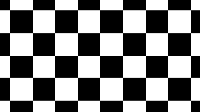
\includegraphics[width=13.3em]{RadialBlurInoOriginalImage}}
\put(92.5,-343){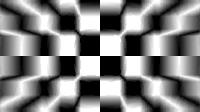
\includegraphics[width=13.3em]{RadialBlurInoRadialBlur30AAOFF}}
\put(314.5,-343){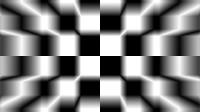
\includegraphics[width=13.3em]{RadialBlurInoRadialBlur30AAON}}
\put(92.5,-486){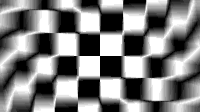
\includegraphics[width=13.3em]{RadialBlurInoTwistBlur20Twist45AAOFF}}
\put(314.5,-486){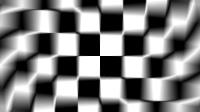
\includegraphics[width=13.3em]{RadialBlurInoTwistBlur20Twist45AAON}}
\put(26,-50){\normalsize{Original Image}}
\put(26,-67){\normalsize{(200x112pixel)}}
\put(89,-221){\normalsize{Anti Alias \ \ OFF}}
\put(311,-221){\normalsize{Anti Alias \ \ ON}}
\put(26,-249){\normalsize{Radial}}
\put(26,-267){\normalsize{(Blur 30)}}
\put(26,-382){\normalsize{Twist}}
\put(26,-400){\normalsize{(Blur 20}}
\put(32,-418){\normalsize{Twist 45)}}
\end{picture}\\[12.65em]

\end{document}